\section{Quickstep Background}\label{sec:sys-background}
In this section we provide a brief background of \sys{} and its implementation of different pipelining strategies. 
\sys{} is designed with a goal to get high performance for in-memory analytic workloads.
One of the techniques used by \sys{} to get high performance is through large intra-operator parallelism. 

\sys{} uses a cost-based optimizer to generate query plans. 
Joins in \sys{} use non-partitioned hash based implementation. 
The operators in \sys{} process a batch of input tuples, rather than one tuple at a time. 
Prior work~\cite{hyper-pipelining} has shown that the vectorized style processing outperforms tuple-at-a-time processing technique.

\sys{} uses an abstraction called \textit{\wo{}s}, which represents the relational operator logic that needs to be executed on a specified input.
The work done for a query is broken up in a series of \wo{}s.
These \wo{}s can be executed independently and in parallel.

\sys{} has two kinds of threads - a scheduler thread and several worker threads.
The worker threads execute these \wo{}s.
The scheduler thread coordinates the execution of \wo{}s which includes dispatching the \wo{}s to worker threads and monitoring the progress of query execution.
Once assigned a \wo{}, the worker thread executes it until its completion. 

\subsection{Managing Storage in \sys{}}
\sys{} supports a variety of storage formats such as row store, column store with the optional support of compression. 
The data in a table is horizontally partitioned in small independent storage blocks, as proposed in some earlier designs~\cite{quickstep-storage, quickstep-system}. 
The size of each storage block is fixed, yet configurable.
The intermediate output of relational operators (e.g. filter) is stored in temporary output blocks, which follow a similar design as the storage blocks of the base tables. 

Each relational operator \wo{} has a unique set of input, described based on the semantics of the operator.
For instance, a select \wo{}'s input consists of a storage block and a filter predicate.
A probe join hash table \wo{}'s input is made up of a pointer to the hash table and a probe input block.
A \wo{} execution involves reading the input(s), applying the relational operator logic on the input(s) and writing the output to a temporary block.\footnote{Output of majority of the operators is represented in the form of storage block, except when the output itself is a data structure like hash table; in the case of a build hash operator, or hash-based aggregation operators.}

\sys{} maintains a thread-safe global pool of partially filled temporary storage blocks.
During a \wo{} execution, a block is \textit{checked out} from the pool, output gets written to the block, and it is returned to the pool at the end of the execution. 
Therefore a block is used by atmost one operator \wo{} simultaneously. 
This approach has two benefits: first, we maintain locality of output block when output gets written to it and second, by reusing output blocks memory framgmentation is minimized. 

\subsection{Pipelining Implementation in \sys{}}
\sys{}'s implementation of pipelining is at a block level.
As described earlier, the output of a relational operator \wo{} is stored in temporary blocks.
As soon as a block is full, it is deemed ready for pipelining.
The scheduler receives a signal as soon as an intermediate output block gets filled, after which it dispatches a \wo{} for the consumer operator for execution.\footnote{All partially filled blocks are pipelined at the end of the operator's execution.}


\subsection{Pipelining and Scheduling}\label{ssec:system-scheduling}
The scheduler for \sys{} can implement different scheduling strategies that can have an impact on the sequence in which different \wo{}s for different operators are executed.
We view pipelining and non-pipelining strategies as manifestation of two different scheduling strategies. 

\begin{figure}[t]
	\centering 
	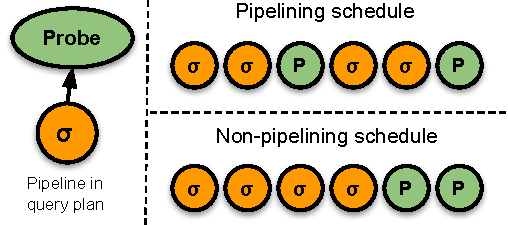
\includegraphics[width=0.5\textheight]{pipeline/figures/Pipe-Nopipe-schedules}
	\caption{\textbf{Interplay between scheduling strategies and pipelining behavior. A sample pipeline of a filter operator ($\sigma$) and a probe operator (P) for a hash join is shown on the left. On the right are two possible interleaving of the \wo{}s of these two operators, resulting in pipelining and non-pipelining schedules}}
	\label{fig:pipelining-schedules}
\end{figure}

For pipelining behavior, a consumer operator \wo{} is scheduled as soon as it is available.
For the non-pipelining behavior, a consumer operator \wo{} is not scheduled until all the corresponding producer \wo{}s have finished execution. 

The implementation of \sys{} scheduler allows to write more sophisticated scheduling policies, such as pipelining implementation with an upper or lower limit on the number of concurrent consumer \wo{}s under execution, or pipelining under a specified memory budget.
To keep our analysis focused, we only discuss the two extremes which are pipelining (eager) and non-pipelining (lazy) strategies.